%/**
% * LaTeX thesis template (main file)
% * @author : Alexander willner <alex@willner.ws>
% * @url    : http://github.com/thesis
% */

% include config ---------------------------------------------------------------
\RequirePackage{pdf14}                 % PDF/A2-b compatibility
%\PassOptionsToPackage{demo}{graphicx} % for faster drafts
% document configuration -------------------------------------------------------
\documentclass[
        %pagesize,              % put paper size information into document
        a4paper,                % use a5paper for ISO A5; use a4paper for ISO A4
        pdftex,                 % PDF output
        %fontsize=12pt,         % font size
        headsepline,            % use headinclude also! (see M. Kohm)
        footsepline,            % use footinclude also! (see M. Kohm)
        %headinclude,            % count head to text body (not to margin)
        %footinclude,            % count foot to text body (not to margin)
        %BCOR8mm,               % set extra margin for book fixation
        headsepline,            % line on the top
        titlepage,              % show a title page
        %draft,                 % show under-/overfull boxes, hide images
        %demo=true,             % faster compile time
        %DIV=calc,              % calculate a nice type area
        %listof=totoc,          % List of Listings to ToC
        %oneside,               % e.g. same headings for odd and even pages
        %oneside=true,          % e.g. same headings for odd and even pages
        %twoside=false,         % e.g. same headings for odd and even pages
        %open=any,              % allows chapters to occur on left hand pages
        %openany,               % allows chapters to occur on left hand pages
        %ngerman,               % German language support
        %numbers=noendperiod    % no number at the end (German DUDEN)
%]{scrbook}
]{book}
% ------------------------------------------------------------------------------


% lang config ------------------------------------------------------------------
\usepackage[english]{babel}                  % English language support
%\usepackage[ngerman,english]{babel}         % German language support
%\usepackage{bibgerm}                        % German bibliography support
%\usepackage[babel,german=quotes]{csquotes}  % German language support
% ------------------------------------------------------------------------------


% basic packages ---------------------------------------------------------------
%\usepackage{tocloft}                         % Tweaks for large ToCs
%\cftsetpnumwidth{2em}                        % Tweaks for large ToCs
%\usepackage[demo]{graphicx}                  % faster compile time
\input{lib/resources/config/default}          % Default config
\usepackage[babel]{csquotes}                  % Biber wants it for babel
\usepackage[export]{adjustbox}                % For boxes around images
\usepackage{needspace}                        % used for embedding listings
%\usepackage{idxlayout}                       % fix index bugs and allow config
% ------------------------------------------------------------------------------

% basic config -----------------------------------------------------------------
\definecolor{LinkColor}{rgb}{0.0,0.2,0.5}     % Link color
\definecolor{MarginColor}{rgb}{0.0,0.2,0.5}   % Margin color
\definecolor{CaptionColor}{rgb}{0.0,0.2,0.5}  % Caption color
\definecolor{disabled}{gray}{0.5}             % Disabled text color
%\addtokomafont{sectioning}{\rmfamily}         % Serifs in headings
%\addtokomafont{sectioning}{\normalfont\scshape\rmfamily\color{CaptionColor}} % Serifs in headings
%\addtokomafont{sectioning}{\normalfont\rmfamily\color{CaptionColor}}        % Serifs in headings
\renewcommand{\lstlistlistingname}{List of Listings}
\renewcommand{\lstlistingname}{Listing}
\renewcommand{\contentsname}{Table of Contents}
\setcounter{secnumdepth}{4}
\setcounter{tocdepth}{2}
% basic config -----------------------------------------------------------------


% local config -----------------------------------------------------------------
\usepackage{pdflscape}
%\usepackage{subfig}
\usepackage{xmpincl}
%\includexmp{an-xmp-file-if-you-like}
\usepackage{enumitem}                   % More compact listings
\usepackage{float}                      % Provides the H float modifier option
% ------------------------------------------------------------------------------


% bibliography -----------------------------------------------------------------
\usepackage[
            style=numeric,%ieee,
            sorting=none,
            backref,
            backend=biber,
            defernumbers=true,
            useprefix=true,
            giveninits=true,
            %maxcitenames=2,
            maxbibnames=99, minbibnames=99,
            %doi=false,isbn=false,url=false,
            ]{biblatex}
\addbibresource{thesis_template.bib}
\defbibheading{empty}{}
\DeclareBibliographyCategory{cited}
\AtEveryCitekey{\addtocategory{cited}{\thefield{entrykey}}}
% ------------------------------------------------------------------------------


% acronyms ---------------------------------------------------------------------
\usepackage{acro}
\acsetup{
            single=false,
            list/sort=true,
            list/template=longtable,
            index/use, %  migh result in 'pdfTeX warning (dest): name... has been referenced but does not exist, replaced by a fixed one'
            pages/display=first,
}
\robustify\footnote%
\robustify\url%

\makeatletter\newif\ifnewacro%
\@ifpackagelater{acro}{2015/08/15}{% version 2.0 or later
\setboolean{newacro}{true}
}{% else hide footnotes and citations
\setboolean{newacro}{false}
\typeout{warning: your acro package is too old (<2.0)}
}%
\makeatother
% ------------------------------------------------------------------------------


% more config ------------------------------------------------------------------
% todo: move to 'basic config'
\usepackage{lmodern}                          % Nicer fonts (for all) - times
\usepackage{mathptmx}                         % Nicer fonts (for all) - times
%\usepackage{scrhack}                         % Fix some scrbook issues
\usepackage{scrlayer-scrpage}                 % before titlesec 
\usepackage{chapterthumb}                     % Fancy thumb index
\usepackage[chapter]{algorithm}               % Nice pseudo code
\usepackage{lettrine}                         % Drop characters, if you like
\renewcommand{\LettrineFontHook}{\color{CaptionColor}}
\usepackage[nohints]{minitoc}                 % ToC for chapters
\dominitoc[n]                                 % ToC: no caption
\renewcommand{\mtcSfont}{\small}              % ToC: small
\usepackage{makeidx}                          % Make an index
\makeindex                                    % Make an index
% ------------------------------------------------------------------------------

% chapter layout ---------------------------------------------------------------
%\usepackage[Sonny]{fncychap}                  % Nice chapter header
%\ChNameVar{\vspace*{-1in}\Large\rmfamily\vspace*{-2in}}   % Fancy chapter with serifs
%\ChTitleVar{\color{CaptionColor}\Large\rmfamily\scshape}  % Fancy chapter with serifs
\usepackage[clearempty]{titlesec}            % Suppress header and footer for empty pages
\setlength{\headheight}{1.1\baselineskip}
\titleformat{\chapter}[display]
  {\scshape\huge\color{CaptionColor}}
  {\filleft\Large\chaptertitlename~\thechapter}
  {2.5ex}
  {\titlerule\vspace{1ex}\filleft}
  [\vspace{1ex}\titlerule]
% ------------------------------------------------------------------------------

% spqueezing -------------------------------------------------------------------
%\usepackage{etoolbox}
%\makeatletter
%\patchcmd{\AC@@acro}
%  {\dotfill\pageref{acro:#1}}
%  {\nobreak\leaders\hbox{$\mkern -7mu \mkern \@dotsep mu\hbox{.}\mkern \@dotsep mu \mkern 7mu$}%
%   \hfill\nobreak\makebox[1.3em][r]{\pageref{acro:#1}}}
%  {}
%  {}
%\makeatother
% ------------------------------------------------------------------------------


% wall papger / logo on first page ---------------------------------------------
 \usepackage{wallpaper}
 \newlength\cornerXoffset%
 \newlength\cornerYoffset%
 \setlength\cornerXoffset{2cm}        % X
 \setlength\cornerYoffset{2cm}        % Y
 \newcommand\ThisLROffsetCornerWallPaper[2]{%
  \AddToShipoutPicture*{%
    \AtPageLowerLeft{%
      \parbox[b]{\paperwidth-\cornerXoffset}{%
        \hfill \includegraphics[width=#1\paperwidth,height=#1\paperheight,%
        keepaspectratio]{#2}%
        \vspace{\cornerYoffset}\null%
      }
    }
  }
 }
% ------------------------------------------------------------------------------


% page layout ------------------------------------------------------------------
%  \usepackage[ % Optional page bleed
%    cross, # some printing services might not like it others may require it...
%    center,
%    width=216mm, % A4 + 6mm
%    height=303mm % A4 + 6mm
%  ]{crop}
\usepackage[pass,a4paper]{geometry}
%\usepackage[marginparwidth=.7in, marginparsep=0.2in]{geometry}
%\geometry{a4paper, bottom=4cm}
% \renewcommand{\topfraction}{0.9}
% \renewcommand{\bottomfraction}{0.9}
% \renewcommand{\textfraction}{0.07}         % allow minimal text w. figs
% \renewcommand{\floatpagefraction}{0.7}     % require fuller float pages
% \renewcommand{\dblfloatpagefraction}{0.7}  % require fuller float pages
% \renewcommand{\dbltopfraction}{0.9}        % fit big float above 2-col. text
% \renewcommand{\textfloatsep}{5mm}
% \setcounter{topnumber}{2}
% \setcounter{bottomnumber}{2}
% \setcounter{totalnumber}{4}                % 2 may work better
% \setcounter{dbltopnumber}{2}               % for 2-column pages
% ------------------------------------------------------------------------------


% hyperlinks (almost last package) ---------------------------------------------
\usepackage{hyperxmp}                 % Semantic meta data (RDF/XMP)
%\pdfminorversion=4                   % PDF/A compatbility
%\pdfobjcompresslevel=0               % PDF/A compatbility
%\pdfcompresslevel=0                  % PDF/A compatbility
\usepackage[pdftex,                   % Hyperlinks in PDFs
pdfa=true,                            % PDF/A compatbility (fix hyperlink with ghostscript)
pdfapart=1,                           % PDF/A compatbility
unicode=true,                         % PDF/A compatbility
raiselinks=true,			                % calculate real height of the link
breaklinks,                           % break links
%backref=page,                        % backlinks in bibliography (section, slide, page, none)
%pagebackref=true,                    % backlinks in bibliography
hyperindex=true,                      % backlinkex index
linktocpage=true,                     % ToC links pages
bookmarks=true,                       % Bookmarks for PDF viewers
bookmarksopen=true,                   % Open bookmarks
bookmarksopenlevel=2,                 % How many levels to open
bookmarksnumbered=true,               % Numbers in the bookmarks
bookmarkstype=toc,                    % Type of bookmark
plainpages=false,                     % Anchors even on plain pages?
pageanchor=true,                      % Pages are linkable
pdfstartview=FitH,                    % Open document with Fit Width
pdfpagelabels=true,                   % set PDF page labels
pdfpagemode=UseOutlines,              % Show bookmarks in viewer
colorlinks,                           % Show colored links
linkcolor=LinkColor,                  % Link color
urlcolor=LinkColor,                   % URL color
anchorcolor=LinkColor,                % Anchor color
citecolor=LinkColor,                  % Cite color
menucolor=LinkColor,                  % Menu color
hypertexnames=true                    % Whatever ;)
]{hyperref}                           % Use hyperlinks
%\renewcommand*{\backref}[1]{[cited at page #1]} % Show formatted backlinks
\usepackage{bookmark}                 % Manually add PDF bookmarks
\hypersetup{keeppdfinfo}              % fix for hyperxmp, however, breaks PDF/A compliance
% ------------------------------------------------------------------------------


% cleveref with fixes ----------------------------------------------------------
\usepackage{cleveref}                 % To ref footnotes twice (use after hyperref)
\crefformat{footnote}{#2\footnotemark[#1]#3}
% ------------------------------------------------------------------------------


% glossary (last package) ----------------------------------------------------
\usepackage[xindy,nonumberlist,toc]{glossaries}
\input{thesis_template.glos.tex}
\setglossarystyle{altlist}
\renewcommand*{\glsgroupskip}{}
\makeglossaries%
% ------------------------------------------------------------------------------


% meta data --------------------------------------------------------------------
% meta data --------------------------------------------------------------------
\newcommand{\metaType}{PhD of templates}
\newcommand{\metaTypeShort}{Dr.-Tmpl.}
\newcommand{\metaWhy}{To get the degree in}
\newcommand{\metaHowFinal}{Submitted}
\newcommand{\metaHowNonFinal}{Draft}
\newcommand{\metaBoard}{Board}
\newcommand{\metaSubmitted}{Presented by}
\newcommand{\metaDate}{30.09.2021}
\newcommand{\metaDateEn}{16.~June~2020}
\newcommand{\metaDateExam}{\metaDate}
\newcommand{\metaNumber}{2020--06}
\newcommand{\metaTitleLayouted}{Sophisticated Template\\for a Thesis}
\newcommand{\metaTitle}{Exploration of methods for in-hand slip detection with an event-based camera during pick-and-place motions}
\newcommand{\metaTitleShort}{Thesis Template}
\newcommand{\metaDegree}{MTA}
\newcommand{\metaBirthplace}{Born in Foo Bar}
\newcommand{\metaAuthor}{First Last}
\newcommand{\metaAuthorMail}{first.last@example.org}
\newcommand{\metaKeywords}{Foo, Bar, First, Last}
\newcommand{\metaSubject}{Template Subject}
\newcommand{\metaUniversity}{Template University}
\newcommand{\metaFaculty}{Template Faculty}
\newcommand{\metaDepartment}{Template Department}
\newcommand{\metaCitycode}{12345}
\newcommand{\metaCity}{Berlin}
\newcommand{\metaCountry}{Country}
\newcommand{\metaURL}{http://example.org}
\newcommand{\metaChair}{Chair}
\newcommand{\metaChairName}{Prof.\ Dr.-Ing.\ Goo Gl}
\newcommand{\metaChairUniversity}{Industry}
\newcommand{\metaReviewer}{Reviewer}
\newcommand{\metaFirstReviewerName}{Prof.\ Dr.-Ing.\ Foo Bar}
\newcommand{\metaFirstReviewerUniversity}{Example University}
\newcommand{\metaSecondReviewerName}{Prof.\ Dr.\ Bar Foo}
\newcommand{\metaSecondReviewerUniversity}{Another University}
\newcommand{\metaThirdReviewerName}{Dr.\ John Smith}
\newcommand{\metaThirdReviewerUniversity}{My University}
\newcommand{\metaFourthReviewerName}{{\color{gray}Dr.\ Jon Doe}}
\newcommand{\metaFourthReviewerUniversity}{{\color{gray}BAR}}


\newcommand{\metaAuthorShort}{\metaAuthor}
\newcommand{\metaConference}{Conference}
\newcommand{\metaConferenceArea}{Area}
\newcommand{\metaDedication}{\scriptsize{Dedicated to my beloved family.}}
% ------------------------------------------------------------------------------

\input{lib/resources/config/pdfmetadata}
% ------------------------------------------------------------------------------


% final fixes ------------------------------------------------------------------
\righthyphenmin=2
\tolerance=2000
\emergencystretch=10pt
% ------------------------------------------------------------------------------

% PDF/A color profile ----------------------------------------------------------
\immediate\pdfobj stream attr{/N 3}  file{lib/resources/pdfa/srgb.icc}% chktex 1
\pdfcatalog{%
/OutputIntents [ <<
/Type /OutputIntent
/S/GTS_PDFA1
/DestOutputProfile \the\pdflastobj\space 0 R
/OutputConditionIdentifier (sRGB IEC61966-2.1)% chktex 8
/Info(sRGB IEC61966-2.1)% chktex 8 chktex 36
>> ]
}
% ------------------------------------------------------------------------------
     % inlcude general configuration
\DeclareAcronym{ABAC}{short={ABAC}, long={Attributed Based Access Control}, cite={li2002design,Yuan2005}}
\DeclareAcronym{DBpedia}{short={DBpedia}, long={DBpedia}, cite={Auer2007}, long-post={\acroiffirstT{\footnote{\url{http://dbpedia.org}}}}, first-style = long, tag=exclude}
%\DeclareAcronym{PLC}{short={PLC}, long={Programmable Logic Controller}}
%\DeclareAcronym{}{short={}, long={}}
%\DeclareAcronym{}{short={}, long={}, short-indefinite={an},  long-indefinite={an}, cite={}, long-post={\acroiffirstT{\footnote{\url{https://}}}}, first-style = long, tag=exclude}
%\DeclareAcronym{Swoogle}{short={Swoogle}, long={}, cite={ding2004swoogle}, long-post={\acroiffirstT{\footnote{\url{http://swoogle.umbc.edu}}}}}
       % inlcude acronyms
\DeclareUnicodeCharacter{0301}{}       % fixing an UTF-8 encoding issue
%\usepackage[norefs,nocites]{refcheck} % useful, but not working with cref
%\usepackage[doublespacing]{setspace}  % useful for reviewing a printout
%\PassOptionsToPackage{cmyk}{xcolor}   % PDF/A compatibility, skipped
%\usepackage[a-2b]{pdfx}               % PDF/A compatibility, skipped
\newcommand{\isFinal}{true}            % Modify e.g. the title page
\AddLayersToPageStyle{@everystyle@}{chapterthumb}
\addtokomafont{chapterthumb}{\bfseries}
% ------------------------------------------------------------------------------


% include only required files for faster building ------------------------------
%\includeonly{src/03_requirements,src/06_implementation}
% ------------------------------------------------------------------------------


% begin thesis -----------------------------------------------------------------
\begin{document}
    \frontmatter
    \pagestyle{empty}
    \pagenumbering{alph}
    \pdfbookmark{Title}{title}
\begin{titlepage}
\newgeometry{left=35mm, right=35mm, top=35mm, bottom=35mm}


\begin{center}
\vspace*{1cm}
\large{Master Thesis}
\\
\vspace*{1cm}
\textbf{\LARGE{\metaTitle}}\\
\normalsize

\vspace*{1cm}
\Large{Albert Bhagwan Bahrunani}
\\
\vspace*{1cm}
\large{Matriculation Number: 046319}
\\
\large{Email: albert.bhagwan@gmail.com}
\vspace*{1cm}

\begin{figure}[h]
	\centering
	
\includegraphics[width=0.4\textwidth]{resources/images/TU-Berlin-Logo.png}
\end{figure}

\vspace*{1cm}
\large{Robotic Interactive Perception}
\\
\large{Institut für Technische Informatik und Mikroelektronik}
\\
\large{Fakultät Elektrotechnik und Informatik}
\\
\large{Technische Universität Berlin}
\\


\end{center}

\ifthenelse{\equal{\isFinal}{true}}{

\vspace*{2cm}
\large{Supervised by: Prof. Dr. Guillermo Gallego}

\vspace*{1,9cm}
\large{\metaDate}
\vspace*{0,9cm}

}{
\vspace*{6cm}
}

\restoregeometry%
\end{titlepage}

    \cleardoublepage\input{src/00_deposition}
    \cleardoublepage

    \pagestyle{scrheadings}
    %\lohead[]{}
    \pagenumbering{roman}
    \setcounter{page}{1}
    \pdfbookmark{Acknowledgments}{acknowledgments}
\chapter*{Acknowledgments}

First, I would like to thank my supervisor, Prof. Dr. Guillermo Gallego, for giving me the opportunity to work on a cutting edge robotics topic and providing me always with his best advice and the necessary knowledge and tools.\\

Additionally, I really appreciate the advice and support of Prof. Dr. Marc Toussaint, making us available their laboratory and their code.\\

Moreover, special thanks to Dr. Jeremy L Wyatt for the regular feedback on the progress of the project.\\

Then, I would also like to thank my colleague, Suman Ghosh, for working on the project side-by-side and providing help whenever I needed it.\\

Finally, I want to thank my family and friends for their unconditional support at all times.

\vspace{0.5in}
\begin{flushright}
  \metaCity, \metaDate
\end{flushright}
\cleardoublepage{}
    \pdfbookmark{Abstract}{abstract}
\chapter*{Abstract}

Pick-and-place motions executed by robotic arms are widely used in the industry and they need to be performed effectively and without errors, such as slips and grasp failures. Concretely, rotational slip may occur when the object is grasped away from its center of mass and may cause issues when placing it due to its change of orientation. In this thesis, this problem is tackled using an event-based camera, which is designed to trigger an input event only the change in illumination at a specific image location crosses a predefined threshold. This enables us to exclude redundant information from static parts of the scene and build systems with low latency, high dynamic range, high temporal resolution and low power consumption.\\

The topic of slip detection in manipulation tasks using event-based cameras is novel. Only a handful of papers in the literature tackle this problem and most of them do not perform as large motions as this thesis considers, typical of pick-and-place scenarios.\\

The main contributions of this work are the design of the data acquisition system and some exploration on data processing methods to infer properties of the scene (motion, slip, etc.) from the data acquired by the platform. In terms of the experiment setup, the event-based camera (DAVIS 346) is mounted to the robotic arm (Panda) with the designed reconfigurable camera mount, offering an external view of the contact between the object and the two-finger parallel gripper used as end-effector. With this setup some small sets of data were recorded, containing slip and non-slip cases during pick-and-place motions with different objects and backgrounds. Since this is an exploratory topic and data is therefore scarce, the approach to data processing consists of feature engineering. To this end, events are processed to investigate the usefulness of alternative representations, such as event histograms and optical flow, to detect slip. Concretely, the ratio between the events coming from the object and the whole image and the vertical absolute mean velocity of the object are considered as one-dimensional signals, which can be thresholded to determine whether a slip is happening or not. In order to discriminate the events related to the object from the background, several solutions are proposed and compared.\\

The results show that indeed, both signals are informative for slip detection, presenting some limitations to generalize for different objects and backgrounds. In the end, some possible solutions to the detailed limitations are proposed.\\

\textbf{Keywords:} Event-based cameras, slip detection, manipulation, pick-and-place motions, event processing

\cleardoublepage
\begin{otherlanguage}{ngerman}
\pdfbookmark{Zusammenfassung}{Zusammenfassung}
\chapter*{Zusammenfassung}%

Pick-and-Place-Bewegungen, die von Roboterarmen ausgeführt werden, sind in der Industrie weit verbreitet und müssen effektiv und ohne Fehler, wie z. B. Schlupf und Greiffehler, durchgeführt werden. Konkret kann es zu einem Drehschlupf kommen, wenn das Objekt außerhalb seines Schwerpunkts gegriffen wird, was zu Problemen bei der Platzierung führen kann, da sich die Ausrichtung des Objekts ändert. In dieser Arbeit wird dieses Problem mit einer ereignisbasierten Kamera angegangen, die so konzipiert ist, dass sie nur dann ein Eingabeereignis auslöst, wenn die Beleuchtungsänderung an einer bestimmten Bildposition einen vordefinierten Schwellenwert überschreitet. Dies ermöglicht es uns, redundante Informationen aus statischen Teilen der Szene auszuschließen und Systeme mit geringer Latenz, hohem Dynamikbereich, hoher zeitlicher Auflösung und geringem Stromverbrauch zu entwickeln.\\

Das Thema der Schlupfdetektion bei Manipulationsaufgaben mit ereignisbasierten Kameras ist neu. In der Literatur gibt es nur eine Handvoll Arbeiten, die sich mit diesem Problem befassen, und die meisten von ihnen behandeln keine so großen Bewegungen wie die in dieser Arbeit betrachteten, die für Pick-and-Place-Szenarien typisch sind.\\

Die wichtigsten Beiträge dieser Arbeit sind der Entwurf des Datenerfassungssystems und einige Untersuchungen zu Datenverarbeitungsmethoden, um aus den von der Plattform erfassten Daten Eigenschaften der Szene (Bewegung, Schlupf usw.) abzuleiten. Die ereignisbasierte Kamera (DAVIS 346) ist mit der neu konfigurierbaren Kamerahalterung am Roboterarm (Panda) angebracht und bietet eine externe Sicht auf den Kontakt zwischen dem Objekt und dem als Endeffektor verwendeten Zweifingergreifer. Mit diesem Aufbau wurden einige kleine Datensätze aufgezeichnet, die Fälle von Schlupf und Nicht-Schlupf bei Pick-and-Place-Bewegungen mit verschiedenen Objekten und Hintergründen enthalten. Da es sich um ein exploratives Thema handelt und die Daten daher spärlich sind, besteht der Ansatz zur Datenverarbeitung im Feature Engineering. Zu diesem Zweck werden Ereignisse verarbeitet, um die Nützlichkeit alternativer Darstellungen, wie Ereignis-Histogramme und optischer Fluss, zur Erkennung von Schlupf zu untersuchen. Konkret werden das Verhältnis zwischen den Ereignissen, die vom Objekt und dem gesamten Bild stammen, und die vertikale absolute Durchschnittsgeschwindigkeit des Objekts als eindimensionale Signale betrachtet, für die ein Schwellenwert festgelegt werden kann, um festzustellen, ob ein Schlupf vorliegt oder nicht. Um die Ereignisse, die mit dem Objekt zusammenhängen, vom Hintergrund zu unterscheiden, werden einige Lösungen vorgeschlagen und verglichen.\\

Die Ergebnisse zeigen, dass beide Signale in der Tat informativ für die Erkennung von Rutschen sind, wobei die Verallgemeinerbarkeit für verschiedene Objekte und Hintergründe eingeschränkt ist. Am Ende werden einige mögliche Lösungen für die detaillierten Einschränkungen vorgeschlagen.\\

\textbf{Schlüsselwörter:} Ereignisbasierte Kameras, Schlupferkennung, Manipulation, Pick-and-Place-Bewegungen, Ereignisverarbeitung

\end{otherlanguage}


\cleardoublepage
\cleardoublepage

    \phantomsection
    % Change the depth for review
\pdfbookmark{Table of Contents}{toc}
\renewcommand{\contentsname}{Table of Contents}
\tableofcontents

\cleardoublepage
\phantomsection\addstarredchapter{\listfigurename}
\listoffigures

\cleardoublepage
\cleardoublepage

    \mainmatter
    %\lohead[\putchapterthumb]{\putchapterthumb}
    \pagenumbering{arabic}
    \setcounter{page}{1}
    %\linenumbers
    \acresetall%
    \cleardoublepage\chapter{Introduction}\label{sec:introduction}

\section{Background and Motivation}

As a student of a double MsC in Industrial Engineering and Automatic Control and Robotics with experience in research in robotics field, my aim was to work on a thesis in a cutting edge topic about robotics which is applicable to the industry. After contacting my supervisor, I got the opportunity to work on part of a project called "Online in-hand object tracking and grasp failure detection with an event-based camera", which is a Amazon Research Awards Proposal.\\

The two main expected outcomes of this project are the creation of a dataset using event-based cameras for manipulation and the design of an algorithm capable to detect grasp failure and object slipping and recover from it in real-time. This project is really relevant for Amazon, as the automation of the package preparation requires to effectively perform pick and place motions by robotic arms. Actually, every year Amazon organizes the Amazon Robotics Challenge, where several teams try to solve a proposed problem. Concretely, they have asked the teams to develop an algorithm to grasp, recognize and place objects in clutter.\\

The problem of object tracking during manipulation to detect grasp failure and object slipping requires of in-hand object perception, which typically is approached with tactile sensing. However, tactile sensors may have disadvantages in industrial settings due to wear and a lack of long-term robustness. Additionally, they are expensive and provide only limited local information to infer the motion of objects that extend far beyond the contact region. This is why in this project event-based cameras, that provide an external view of the grasping operation, are explored as a novel alternative technology for high-speed in-hand object tracking, as for real-time grasping failure mitigation a fast detection is required.

\section{Objectives}

The project "Online in-hand object tracking and grasp failure detection with an event-based camera" is planned to be completed in at least 1 year, and it has started at the same time as this thesis, i.e. in April 2021. Therefore, this thesis is meant to describe the initial results of this project, being the concrete objectives:

\begin{itemize}
	\item Setup the experimental environment: robot, gripper, event-based camera and objects to be manipulated.
	\item Setup the software to execute pick and place motions and collect data.
	\item Generate an initial dataset containing slip and non-slip cases in pick and place motions.
	\item Explore of different methods to detect slip cases and compare them.
	\item Build an initial algorithm capable of detecting slip cases in pick and place motions.
\end{itemize}

\section{Assumptions and Scope}

As the thesis is an initial part of the aforementioned Amazon project, for the purpose of this thesis it has been assumed that the pick and place motions happen in a non-cluttered environment, having only one pickable object in the scene. Moreover, the complete trajectory is given, including not only the shape of it, but also the initial and and final positions. Therefore, it is assumed that some external object recognition algorithm will recognize the object to be picked and provide its position. Finally, the there are no obstacles present in the environment, so that the trajectory is collision-free at all moments.\\

In terms of the scope, this study is focused on exploring different kinds of slips and grasping failures during manipulations, but only providing a solution for a particular kind of slip, namely rotational slip, which mainly occurs due to off-centered grasping of the object. In addition, the goal is only to detect such kind of slippage without trying to modify the trajectory with any kind of closed-loop control, which would use the information provided by the detection algorithm.

\section{Outline}

\todo{Cite like this: \Cref{sec:introduction}}

    \cleardoublepage\chapter{Fundamentals and Related Work}\label{sec:sota}

\section{Event-based cameras}

Event cameras ~\cite{gallego2020} are bio-inspired sensors that differ from conventional frame cameras, as instead of capturing images at a fixed rate specified by an external clock (e.g. 30 fps), they asynchronously measure per-pixel brightness changes, and output a stream of events that encode the time, location and sign of the brightness changes.\\

These novel cameras offer attractive properties compared to traditional cameras:

\begin{itemize}
	\item High temporal resolution: events are detected and timestamped with microsecond resolution. Therefore, event cameras can capture very fast motions, without suffering from motion blur, typical of frame-based cameras.
	\item Low latency: each pixel works independently, thus as soon as the change is detected, it is transmitted. This working principle enables event cameras to have minimal latency, e.g. about 10 $\mu$s on the lab bench, and sub-millisecond in the real world.
	\item High Dynamic Range (HDR): the range for event cameras exceeds 120 dB, in comparison to the 60 dB of high-quality, frame-based cameras, making them able to acquire information in challenging illumination conditions.
	\item Low power consumption: as event cameras transmit only brightness changes, removing redundant data, power is only used to process changing pixels, e.g., at the die level, most cameras use about 10 mW.
\end{itemize}

Hence, event cameras have a large potential for robotics and computer vision in challenging scenarios for traditional cameras. Concretely, it is really suitable for highly responsive systems, like manipulation tasks, where a fast perception is required. Actually, the speed advantage of event-based cameras to enable fast closed-loop control has been demonstrated in ~\cite{CL1}, ~\cite{CL2}, ~\cite{CL3}, ~\cite{CL4}. Such low perception latencies provide enough time to respond effectively, for example, to balance a pencil on its tip.\\

This is why, event-based cameras can be an appropriate choice of visual sensor to perform a corrective actions in robot manipulation. However, novel methods are required to process the unconventional output of these sensors in order to unlock their potential. In ~\cite{gallego2020}, a comprehensive overview of the emerging field of event-based vision is provided.

\section{Robotic arms}

A robotic arm is a type of mechanical arm that is programmed to execute a specific task or job quickly, efficiently and extremely accurately. The links of such manipulator are connected generally by motor-driven joints, which allow either rotational motion or translational displacement. These links form a kinematic chain, trying to resemble the functionality of a human arm, where the main joints imitate the shoulder, elbow and wrist. Moreover, end-effectors are devices that are attached to end of a robotic arm and are in charge to interact with the environment, similarly as a human hand would do.\\

These kind of robots are widely used in industrial applications as they are ideal for operations which are repetitive, consistent and require a very high degree of accuracy, as well as for applications in which a human worker might struggle to perform safely. Concretely, articulated robots are the most common types of industrial robots and they consist of at least three rotary joints. In addition, collaborative robots, or cobots, are designed to work in collaboration with humans, presenting lightweight materials, rounded edges, limited speed and force, and sensors combined with software that ensure safe behavior.\\

A robotic arm is characterized mainly by the:

\begin{itemize}
	\item Degrees of Freedom (DoF): number of independent motions in which the end-effector can move, defined by the number of axes of motion of the manipulator. For example, a human arm has seven DoF.
	\item Work envelope: a three-dimensional shape that defines the boundaries that the robot manipulator can reach.
	\item Payload: the maximum payload is the amount of weight carried by the robot manipulator at reduced speed while maintaining rated precision. Nominal payload is measured at maximum speed while maintaining rated precision. These ratings are highly dependent on the size and shape of the payload. 
\end{itemize}

As mentioned, the links in a robotic arm form a kinematic chain, where each joint is controlled by servomotors. For articulated robots, according to the angular position of each joint, the end-effector ends up being in a certain pose, which can be computed using the forward kinematics. However, usually the end-effector's pose is imposed and the controller needs to set the angular positions of the joints, which are obtained using the inverse kinematics of the mechanism.

\section{Related Work}

Prior work on event-based cameras has demonstrated the outstanding capabilities of these sensors for object tracking ~\cite{OT1}, ~\cite{OT2}, ~\cite{gallego2020} and ego-motion estimation ~\cite{EM1}, ~\cite{EM2}, ~\cite{gallego2020}. However, little work has been done on event-based perception for in-hand object tracking and robot manipulation. The scarce literature in the topic is due to the fact that event-based cameras are an emerging technology, still in prototype phase (commercially available only since 2008), and they are costly (thousand USDs) compared to traditional frame-based cameras. Additionally, there is an entry barrier for people to get familiarized with the remarkably different sensing modality and the type of output produced by event-based cameras.\\

In ~\cite{barranco2018} an event-based camera was used as end-effector of a robot arm to acquire data for visual tracking, but not for manipulation. Instead \cite{muthusamy2020} presents a visual servoing method using an event camera and a switching control strategy to explore, reach and grasp an object, in order to complete a manipulation task. However, they only use simple, high-contrast objects (a white cardboard triangle or rectangle). Moreover, ~\cite{huang2021} proposes an event-based robotic grasping framework for multiple known and unknown objects in a cluttered scene, but only providing a fix plan to be executed and not detecting slip or failure during the grasping operation.\\

In terms of slip detection, ~\cite{rigi2018} proposes a novel approach to detect incipient slip according to the contact area between a transparent silicone medium and different objects, using an event-based camera. The experimental setup consists of the robot arm, event-based camera, LED, silicone medium and adjustable camera frame, as depicted in ~\Cref{fig:rigi2018}. Moreover, the high-speed camera is used for validation purposes. In the experiments, the robot arm applies a force to an object perpendicularly to the surface of the silicon medium and afterwards the force from the robot arm was gradually reduced to release the object, in order to induce slip. This approach is not suitable for pick-and-place operations, where the slip occurs during the moving phase and not pushing the object against a deformable medium. Also, the sensor consists of the event-based camera, LED, silicone medium and adjustable camera frame, which are used in a static way, and in our pick-and-place scenario they would have to move attached to the robot, being prone to vibrations.\\

\begin{figure}[h]
    \centering
    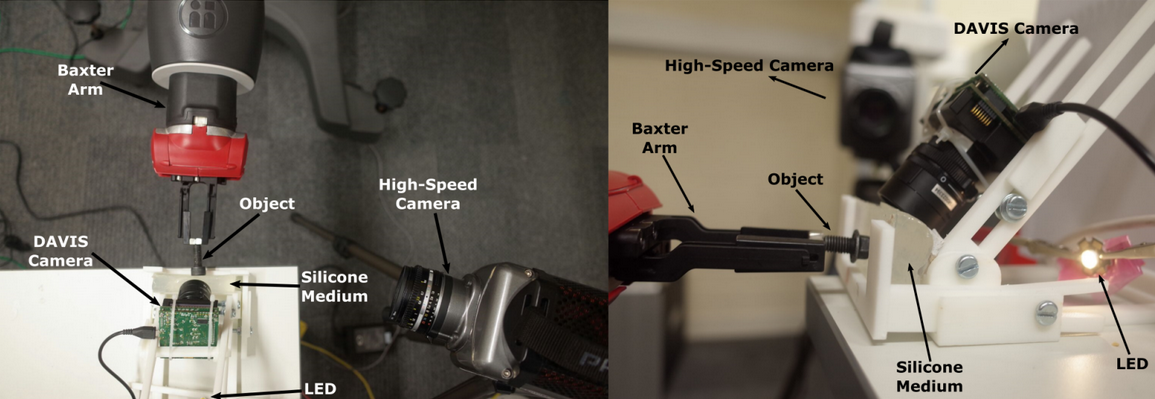
\includegraphics[width=\textwidth]{resources/images/rigi2018}
    \caption{Top-down (left) and sideways (right) views of the experiment setup ~\cite{rigi2018}.}\label{fig:rigi2018}
\end{figure}

Muthusamy et al. \cite{muthusamy2020slip} presents a first study on using an event-based camera with narrow field of view to detect slip during manipulation, but it analyzes only tiny motions. Moreover, it provides a slip suppression strategy regulating the grip force. The experimental setup is formed by the Baxter robot, electric parallel gripper, F/T sensor and a finger with an integrated event-based camera, as shown in ~\Cref{fig:muthusamy2020slip}. The F/T sensor measures six components of force and torque and is used only for validation purposes. In terms of the event-based camera, it observes the object through one of the transparent fingers of the gripper, which limits the information available from the object. The sensor itself moves attached to the gripper in this case, being suitable for pick-and-place operations.

\begin{figure}[h]
    \centering
    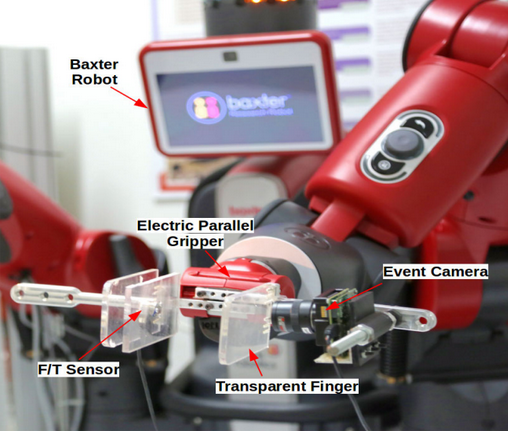
\includegraphics[width=0.7\textwidth]{resources/images/muthusamy2020slip}
    \caption{Experiment setup: Baxter Gripper with event-based finger prototype ~\cite{muthusamy2020slip}.}\label{fig:muthusamy2020slip}
\end{figure}

Another family of sensors widely used in the literature for slip detection are the tactile sensors, which may provide physical signals like the ratio of shear force to normal force, vibration or acceleration. In ~\cite{gelsight2017}, a tactile sensor, called GelSight sensor, is used for measuring geometry and detecting slip. Concretely, both translational and rotational slips are considered during grasp tasks, not complete pick-and-place operations. The GelSight sensor detects slip based on 3 major clues: the relative displacement between the objects and the sensor surface, the shear displacement distribution of the markers on the sensor surface and the change in the contact
area. They perform grasp experiments on 37 daily-use objects, lifting these slowly for 3 cm and then stopping. Each object is lifted 7 to 10 times, with different gripper forces, and the data is manually labeled indicating whether a slip occurred or not during the grasping and lifting process. Moreover, they implement a grasp closed-loop control with the feedback of the GelSight slip detection, using 33 objects and grasping each of them 3 times. If slip is detected the object is released and it is re-grasped with a higher gripping force.\\

In ~\cite{gelsight2018} the tactile information obtained from the GelSight sensor is combined with visual information coming from an external camera (standard webcam). The new setup including this camera is depicted in ~\Cref{fig:gelsight}. In this case a dataset is created including more than 1200 grasp experiments with 94 objects in total (for the train and test sets) and a deep neural network is trained to classify whether in a certain lifting sequence a slip has occured or not. These lifting sequences consider only small vertical motions with a non-textured (uniform) background and, in each grasp, the gripper width is modified in order to provoke slip or even complete failure in the grasp, which is manually annotated. They conclude that the best results are achieved combining tactile and vision information and, when using only vision information, much better results are achieved when the difference of images are taken into account, instead of the raw images. Note that using difference of images coming from a standard camera is a similar paradigm compared to event-based cameras, but these present a lower latency and therefore the feedback is faster.

\begin{figure}[h]
    \centering
    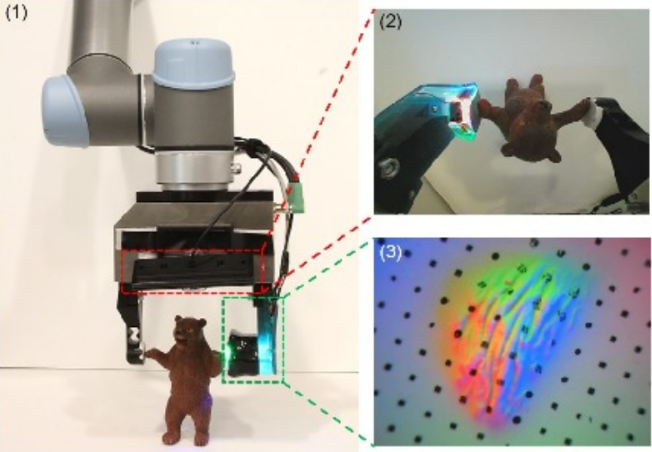
\includegraphics[width=0.7\textwidth]{resources/images/gelsight}
    \caption{(1) Experiment setup: UR5 robot arm with gripper, GelSight sensor and external camera. (2) Image captured by the external camera. (3) Image from GelSight sensor ~\cite{gelsight2018}.}\label{fig:gelsight}
\end{figure}

More work has been done in the combination of tactile and visual information, as in ~\cite{rss2020}, where they designed a Visual-Tactile Spiking Neural Network for rotational slip detection using their NeuTouch tactile sensor and the Prophesee event camera. In the experimental setup, see ~\Cref{fig:rss2020}, they also include 2 RGB cameras (for visualization and validation purposes), one mounted on the end-effector pointing towards the griper and the second one was placed to provide a view of the scene, and 11 OptiTrack cameras were used to collect ground-truth data. OptiTrack is a motion capture system that tracks the motion of some reflective markers attached to, in this case, the end-effector and the object. With this information the relative trajectory of the object with respect to the end-effector can be analyzed to determine whether the slip occurred or not. During the experiments they used a object built with Lego Duplo blocks with hidden masses. One variant was designed to be balanced at the grasp point and the second one, modifying the hidden masses, is unstable to induce rotational slip. Both variants are lifted by 10 cm off the table (in 0.75 s) and then holded, repeating this 50 times for each variant. However, the model was trained only during the first 0.15 s of the lifting phase, as they focus on early slip detection. Additionally, the background scene recorded by the cameras corresponds to a controlled black background.

\begin{figure}[h]
    \centering
    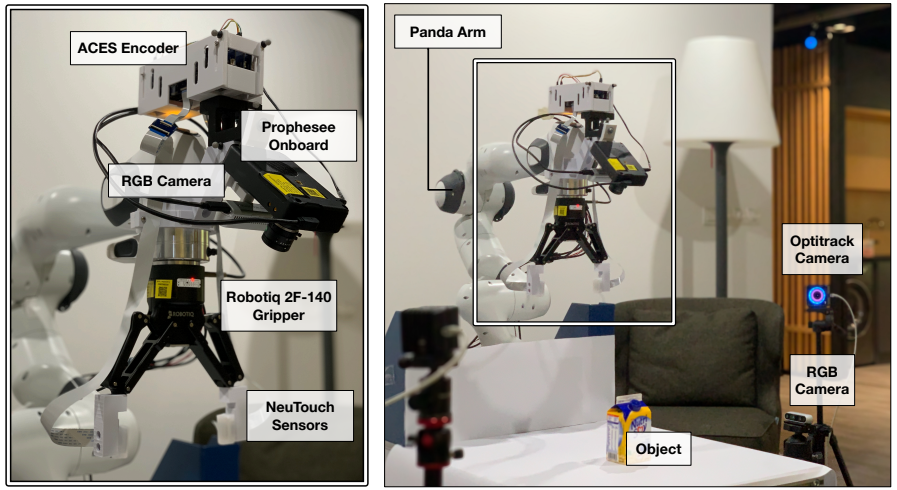
\includegraphics[width=0.95\textwidth]{resources/images/rss2020}
    \caption{Experiment setup: Robot arm, Prophesee event camera, Robotiq gripper, NeuTouch sensors, RGB and OptiTrack cameras ~\cite{rss2020}.}\label{fig:rss2020}
\end{figure}

\section{Conclusion}

Robot arms are widely used for pick-and-place motions and, combined with event-based cameras, which present several advantages compared to conventional frame cameras, they have the potential to form a robust manipulation and slip detection framework.\\

Even though there is some literature tackling this issue, none of them are considering the whole pick-and-place motion to detect slip and instead they are just analyzing tiny motions. Moreover, to make sure the solution generalizes the dataset should also include daily use objects and non-controlled background. When it comes to label the samples, some of the works determine if there is a slip or not by human inspection, however, ideally, having ground-truth data would be more suitable.\\

Most recent works are focusing on combining tactile and vision information, however, in industrial applications tactile sensors may have disadvantages like wear and a lack of long-term robustness. So, considering only visual information, concretely coming from an event-based camera, the placement of the camera in the end-effector should ensure a wide field of view, like in ~\cite{gelsight2018} and ~\cite{rss2020}.\\

In short, the topic of event-based vision for robot manipulation remains largely unexplored and thus offers great opportunities.\\

After having analyzed several experimental setups regarding robot manipulation with slip detection, in the next chapter our particular experimental setup is described.

    \input{src/03_requirements}
    \input{src/04_contrib1}
    \input{src/05_contrib2}
    \cleardoublepage
\chapter{Contribution 3}\label{sec:contrib3}

\section{Introduction}



\section{Conclusion}


    \input{src/07_evaluation}
    \cleardoublepage
\chapter{Conclusions}\label{sec:conclusions}

\section{Summary}

In this work, we perform an exploration of different methods for slip detection during object manipulation in pick-and-place operations using a robot arm with an attached event-based camera, which presents several advantages over frame-based cameras, making it really appropriate for highly responsive systems. Concretely, it has high temporal resolution, low latency, high dynamic range and low power consumption.\\

First, we designed and built the experimental setup, which consists of a robot system, called Panda, including a robot arm and its controller, a two-finger parallel gripper to manipulate the object, the DAVIS 346 camera and a computer connected to it and to the controller of the robot arm and gripper. In addition, to attach the DAVIS 346 to the robot arm and gripper, a mount has been designed and printed, in order to have an external view of the contact between the object and the gripper, while having the camera robustly attached to the robot and offering flexibility when it comes to the position and orientation of the camera with respect to the gripper. Moreover, the software has been set up to execute a desired trajectory during the pick-and-place motion.\\

Then, some small sets of data were recorded, containing slip and non-slip cases during pick-and-place motions with different objects and backgrounds. After analyzing different ways of inducing slip and grasping failures, we focused our efforts in off-centered grasping to produce rotational slip. In total three sets of data have been collected, which have been studied and analyzed iteratively to discover new sources of information that were necessary to be recorded, generating the necessity of recording new sets of data.\\

In terms of the methods tested to determine slip cases, they can be classified in two main groups, depending on the source of information used. On the one hand, the first one considers that whenever a slip occurs, the object moves with respect to the camera (also to the robot arm and gripper), which generates events due to the texture of the object, producing an increase in the number of events in the region where the object is present. To separate the object from the background, three ways have been analyzed and compared, namely, the fixed RoI, the weighted mask and the variable mask approaches. Once the events from the object are separated, the event rate and ratio signals are computed, which can be thresholded to detect slip. On the other hand, a slip can be detected by estimating the motion of the scene through optical flow, which is obtained using EV-FlowNet ~\cite{evflownet}. Whenever, a rotational slip occurs, the object presents mainly vertical motion, that is why the horizontal and vertical absolute mean velocities are computed separately, so that thresholding the vertical one, slip can be detected. To separate the object's motion from the background, in this case, the fixed RoI and weighted mask approaches have been compared.\\

For the ratio signal, the fixed RoI presents several disadvantages, e.g. it needs to be annotated for each experiment, it fails in cases where the object's shape changes significantly from the camera's view and it is not robust to changes in the background's texture. With the weighted mask approach these issues are solved, however the threshold still depends on the object's texture. Moreover, the weighted mask and variable mask approaches present similar results, but the variable mask one is quite brittle and requires of extra computations.\\

On the contrary, for the vertical absolute mean velocity signal, the fixed RoI works robustly in all scenarios, while the weighted mask approach fails in one of the experiments, producing false positives.\\

Both described methods are informative about rotational slip, however, the ratio signal is easier to threshold, as it is bounded between 0 and 1, compared to the vertical absolute mean velocity one, which is not bounded.

\section{Limitations and Future Work}

The designed 1D signals, which were intended to be thresholded and detect slip, are not robust enough to work in different scenarios. The ratio signal is sometimes not enough to differentiate between a non-slip and a slip case and in highly textured backgrounds, the orientation of the motion is not properly estimated, thus, the vertical absolute mean velocity may not be enough to detect slip. All in all, these handcrafted 1D signals are a first step to understand slip detection, but are not enough to generalize in different scenarios and detect slip robustly.\\

There are several ideas that we had in mind, but could not execute them in the time frame of this thesis. First, in Set 2, the camera's angular velocity was recorded along with the other data to compute the motion flow of the scene. The idea behind that is to estimate the background's motion through these known velocities and compare them to the optical flow, in order to detect anomalies between the predicted motion and the real one, being these anomalies, independent motion corresponding to slips.\\

Also, in order to separate the object properly from the background, we tried to identify independently moving objects in the scene, where the background should be identified ideally as a single object and the manipulated object, if there is no slip, it is not a moving object, but if it rotates it should be identified as another independently moving object. We tried to use a novel event-based motion segmentation method ~\cite{motionsegmentation}, but the segmentation was not properly done. Therefore, we assume that the algorithm needs to be fine-tuned to our concrete problem, constraining to the kind of motion we are executing. However, this implies the modification of the motion segmentation code, which is out of the scope of this work.\\

We have seen that the ratio of events and the vertical velocity are informative of slip detection, however, thresholding these signals is not generalizable. Therefore, this information can be used as input to supervised learning methods. Nevertheless, to explore this possibility and be able to train and validate the models, much more data is needed, which includes repeated pick-and-place motions of diverse daily use objects with balanced non-slip and slip cases. Moreover, this dataset should be labeled, which can be done using the motion capture system, i.e. the OptiTrack. To this end, Set 3 was recorded, where the relative pose between the gripper and the object changes when there is a slip. This motion capture system can be used as ground-truth, but not for usual slip detection, as the system is not practical nor flexible to use in general scenarios.\\

Finally, the slip detection problem can be analyzed in non-cluttered environment, picking one object among several objects, which is a more realistic scenario but considered out of the scope of this thesis.\\

Once this rotational slip detection problem is solved, linear slip and other grasping failures should be considered. Moreover, to complete the ARA project, once these slips and grasp failures are detected, the pick-and-place motion should be modified appropriately in order to complete it successfully, using the feedback of the slip and failure detection algorithm.



    \nolinenumbers
    \cleardoublepage

    \appendix
    \pagenumbering{Roman}
    \setcounter{page}{1}
    \input{src/09_appendix}

    \cleardoublepage
    \cleardoublepage
\chapter*{Bibliography}
\mtcaddchapter\addstarredchapter{Bibliography}
\markboth{Bibliography}{Bibliography}
\stepcounter{chapter}
\renewcommand*{\chapterthumbformat}{Bibliography}

\printbibliography[heading=empty,category=cited,sorting=none]



    \backmatter
\end{document}
% ------------------------------------------------------------------------------
